\documentclass[conference]{IEEEtran}
\IEEEoverridecommandlockouts

\usepackage[utf8]{inputenc}
\usepackage[T1]{fontenc}
\usepackage[spanish,es-nodecimaldot,es-noshorthands,es-tabla]{babel}
\usepackage{amsmath,amssymb}
\usepackage{booktabs}
\usepackage{graphicx}
\usepackage{url}
\usepackage{cite}
\usepackage[hidelinks]{hyperref}

\graphicspath{{figuras/}}
\renewcommand{\IEEEkeywordsname}{Palabras clave}
\newcommand{\EunoKruskalP}{$p=0.25$}
\newcommand{\EunoMannRankingTorneoP}{$p=0.09$}
\newcommand{\EunoDivMannP}{$p<0.001$}
\newcommand{\EunoGenVeinticincoTorneoRuletaP}{$p=0.03$}
\newcommand{\EunoGenVeinticincoTorneoRankingP}{$p<0.001$}
\newcommand{\EunoKruskalGenVeinticincoP}{$p<0.001$}
\newcommand{\EunoUltimaMejoraMin}{188}
\newcommand{\EdosExitos}{14}
\newcommand{\EdosExitosOptimoUno}{8}
\newcommand{\EdosExitosOptimoCuatro}{6}
\newcommand{\EdosExitosOptimosDosTres}{0}
\newcommand{\EdosCercaDosTres}{8}
\newcommand{\EdosCercaDosTresErrorMin}{1.6\times10^{-3}}
\newcommand{\EdosCercaDosTresErrorMax}{0.046}
\newcommand{\EdosMedianaUnPunto}{13}
\newcommand{\EdosMedianaDosPuntos}{19}
\newcommand{\EdosMedianaUniforme}{41}
\newcommand{\EdosKruskalGenP}{$p=0.22$}
\newcommand{\EdosKruskalDivP}{$p=0.46$}
\newcommand{\EtresDivMannP}{$p<0.001$}
\newcommand{\EtresFisherP}{$p=0.09$}
\newcommand{\EdosPasosMediana}{34}
\newcommand{\EdosHammingCercanoMin}{9}
\newcommand{\EdosHammingCercanoMax}{20}
\newcommand{\EdosHammingCercanoMediana}{12}
\newcommand{\EdosHammingAzarMediana}{8}
\newcommand{\EtresPasosMediana}{56}
\newcommand{\EtresHammingCercanoMin}{7}
\newcommand{\EtresHammingCercanoMax}{20}
\newcommand{\EtresHammingCercanoMediana}{12}
\newcommand{\EtresHammingAzarMediana}{6}
\newcommand{\EunoMejorRuletaGenVeinticinco}{26.1}
\newcommand{\EunoDivRuletaGenVeinticinco}{0.37}
\newcommand{\EunoMejorTorneoGenVeinticinco}{17.3}
\newcommand{\EunoDivTorneoGenVeinticinco}{0.17}
\newcommand{\EunoMejorRankingGenVeinticinco}{34.4}
\newcommand{\EunoDivRankingGenVeinticinco}{0.44}
\newcommand{\EunoMejorRuletaGenDoscientos}{8.79}
\newcommand{\EunoDivRuletaGenDoscientos}{0.23}
\newcommand{\EunoMejorTorneoGenDoscientos}{9.75}
\newcommand{\EunoDivTorneoGenDoscientos}{0.06}
\newcommand{\EunoMejorRankingGenDoscientos}{7.41}
\newcommand{\EunoDivRankingGenDoscientos}{0.25}
\newcommand{\EunoCruceRankingTorneo}{134}
\newcommand{\EunoCruceRankingRuleta}{134}
\newcommand{\EunoCruceRuletaTorneo}{139}
\newcommand{\EdosSinExito}{16}
\newcommand{\EdosOptimoLocal}{16}
\newcommand{\EdosHammingMin}{5}
\newcommand{\EdosHammingMax}{8}
\newcommand{\EtresSinExito}{8}
\newcommand{\EtresOptimoLocal}{6}
\newcommand{\EtresHammingMin}{2}
\newcommand{\EtresHammingMax}{6}
\newcommand{\EtresUnBitOptimoLocal}{4}
\newcommand{\EtresUnBitSinExito}{4}
\newcommand{\EtresInversionOptimoLocal}{2}
\newcommand{\EtresInversionSinExito}{4}
\newcommand{\ProbDosBits}{0.26}
\newcommand{\ProbConcretosDos}{3.8\times10^{-4}}
\newcommand{\EsperadoConcretosDos}{4}
\newcommand{\ProbConcretosCinco}{1.3\times10^{-8}}
\newcommand{\EsperadoConcretosCinco}{1\times10^{-4}}


\begin{document}

\title{Algoritmo genético binario con interfaz gráfica parametrizable y comparación de sus operadores en Rastrigin, Himmelblau y Peaks}

\author{\IEEEauthorblockN{Sergio Santiago Duarte Rojas}
\IEEEauthorblockA{\textit{Maestría en Ciencias de la Información y las Comunicaciones}\\
Universidad Distrital Francisco José de Caldas\\
ssduarter@udistrital.edu.co}}

\maketitle

\begin{abstract}
Se desarrolló en Python una aplicación de escritorio para un algoritmo genético binario. Desde la ventana se eligen la función, los bits por variable, tres métodos de selección, tres de cruce y tres de mutación, el elitismo, la semilla y los criterios de parada, y las curvas de nivel y de convergencia se actualizan en cada generación. Los operadores se compararon con diez semillas por variante. En Rastrigin de 10 variables el torneo redujo el error más rápido pero perdió la diversidad genotípica (\EunoDivTorneoGenDoscientos{} frente a \EunoDivRankingGenDoscientos{} del ranking lineal), y el valor final no difirió entre métodos (Kruskal-Wallis, \EunoKruskalP). En Himmelblau el cruce de un punto llegó a la tolerancia de $10^{-3}$ en 6 de 10 ejecuciones, sin diferencia significativa entre cruces. En Peaks la mutación bit-flip por bit la alcanzó en las 10 ejecuciones y las otras dos en 6. Las ejecuciones sin éxito quedaron cerca del éxito en el dominio y lejos en bits, lo que es compatible con los acantilados de Hamming de la codificación binaria.
\end{abstract}

\begin{IEEEkeywords}
algoritmo genético, codificación binaria, presión selectiva, operadores genéticos, diversidad genotípica, interfaz gráfica
\end{IEEEkeywords}

\section{Introducción}

Un algoritmo genético (AG) mantiene una población de soluciones candidatas y, generación tras generación, favorece a las mejores y las recombina para producir soluciones nuevas \cite{holland1975,goldberg1989}. No requiere derivadas, y por eso se aplica a funciones multimodales. Su desempeño depende del equilibrio entre exploración y explotación que fijan los operadores y sus parámetros \cite{eiben2015}.

Este trabajo presenta una aplicación con interfaz gráfica en la que todos los parámetros y los nueve operadores se eligen desde la ventana, y la usa para comparar los métodos de selección en Rastrigin, los de cruce en Himmelblau y los de mutación en Peaks, con el protocolo de la guía del curso \cite{guia2026}.

\section{Fundamentos}

\subsection{Codificación y aptitud}

Cada variable $x_j\in[a_j,b_j]$ se representa con $L$ bits, con el más significativo a la izquierda, y el cromosoma concatena los $n$ segmentos en $\ell=nL$ bits. Si $D_j$ es el entero del segmento $j$,
\begin{equation}
x_j=a_j+(b_j-a_j)\,\frac{D_j}{2^L-1},\qquad L=\left\lceil\log_2\!\left(\frac{b-a}{\varepsilon}+1\right)\right\rceil,
\end{equation}
donde la segunda expresión da los bits necesarios para una precisión $\varepsilon$ \cite{michalewicz1996}. El AG siempre aumenta la aptitud $F$, con $F=f$ al maximizar y $F=-f$ al minimizar.

\subsection{Funciones de prueba}

Rastrigin, $f(\mathbf{x})=10n+\sum_{i=1}^{n}[x_i^2-10\cos(2\pi x_i)]$ en $[-5.12,5.12]^n$, tiene una rejilla regular de mínimos locales y el mínimo global 0 en el origen. Himmelblau, $f(x,y)=(x^2+y-11)^2+(x+y^2-7)^2$ en $[-5,5]^2$, tiene cuatro mínimos globales de valor 0 \cite{surjanovic}. Peaks, la función \texttt{peaks} de MATLAB en $[-3,3]^2$, tiene el máximo global 8.1062 en $(-0.0093, 1.5814)$ rodeado de máximos y mínimos locales \cite{peaks}.

\subsection{Operadores}

La ruleta elige al individuo $i$ con probabilidad $p_i=F_i'/\sum_j F_j'$, donde $F_i'=F_i-F_{\min}+10^{-6}$ desplaza la aptitud para que sea positiva. El torneo toma $k$ individuos al azar y gana el de mayor aptitud, de modo que $k$ fija la presión selectiva. El ranking lineal ordena la población y asigna al rango $r_i$ (1 para el peor, $N$ para el mejor)
\begin{equation}
p_i=\frac{1}{N}\left[(2-s)+2(s-1)\frac{r_i-1}{N-1}\right],\qquad 1\le s\le 2,
\end{equation}
que depende del orden y no del valor de la aptitud \cite{eiben2015}.

Con probabilidad $P_c$ cada pareja se cruza sobre el cromosoma completo. El cruce de un punto intercambia las colas a partir de un corte, el de dos puntos intercambia el segmento entre dos cortes y el uniforme decide bit a bit de qué padre copia cada hijo, con probabilidad $p_0$ \cite{syswerda1989}. La mutación bit-flip por bit invierte cada bit con probabilidad $P_m$ y cambia en promedio $\ell P_m$ bits por hijo. La mutación de un bit invierte una sola posición con probabilidad $P_{mi}$ por individuo, y la inversión de segmento invierte, con la misma probabilidad, el orden de los bits entre dos posiciones. Con elitismo, los $e$ mejores pasan intactos a la generación siguiente y la curva del mejor no empeora. La ejecución se detiene al alcanzar $T$ generaciones, cuando el error respecto al óptimo conocido baja de una tolerancia o cuando el mejor no mejora en $G$ generaciones. Si $q_k$ es la fracción de cromosomas con un 1 en la posición $k$, la diversidad genotípica $\mathcal{D}=\frac{1}{\ell}\sum_{k}4q_k(1-q_k)$ vale 1 con cada bit repartido por mitades y 0 con todos los cromosomas iguales. Mide cuánta exploración le queda a la población, y su caída temprana indica convergencia prematura.

\section{Diseño de la aplicación}

La aplicación está escrita en Python con NumPy \cite{harris2020}, PySide6 \cite{pyside6} y Matplotlib \cite{hunter2007}, y sigue la separación de la guía entre motor, controlador y vista. El motor no importa nada de la interfaz y se ejecuta igual desde un guion. Cada operador es una función registrada en un diccionario de su módulo, de modo que uno nuevo se agrega sin tocar la interfaz. El controlador valida cada entrada y muestra un mensaje con el rango esperado, lanza el AG en un hilo aparte que se puede pausar, reanudar o detener, y redibuja la población cada 50 ms y la convergencia cinco veces por segundo con la última generación. Al elegir la función se cargan su tipo, su dominio y su óptimo, y al elegir un operador aparecen solo sus parámetros (Fig.~\ref{fig:interfaz}). Con varias ejecuciones, cada una usa la semilla siguiente y se informan la media y la desviación estándar del mejor valor final, exportables a CSV. Además de las tres funciones de la tarea trae siete de GEATbx \cite{geatbx} y una personalizada que se escribe como expresión de $x_1,\dots,x_n$, y se distribuye también como ejecutable de Windows hecho con PyInstaller \cite{pyinstaller}, que no requiere instalar Python.

\begin{figure*}[!t]
\centering
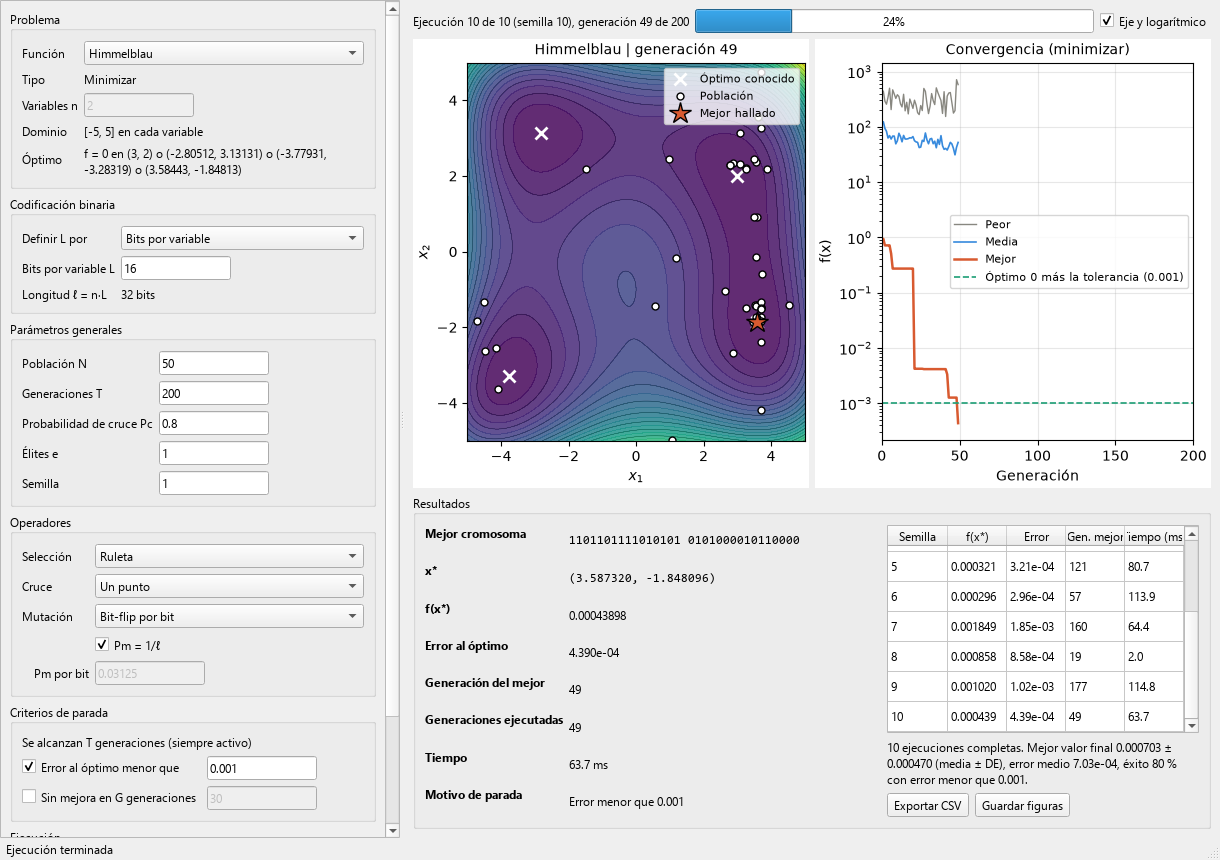
\includegraphics[width=0.83\textwidth]{interfaz_himmelblau.png}
\caption{Ventana al terminar diez ejecuciones en Himmelblau con ruleta, cruce de un punto y bit-flip por bit. A la izquierda, parámetros y operadores. A la derecha, curvas de nivel con la población, convergencia en escala logarítmica, mejor cromosoma decodificado y tabla por ejecución con su resumen.}
\label{fig:interfaz}
\end{figure*}

La comprobación del motor reproduce los ejemplos de la guía, el óptimo de cada función y el mismo resultado con la misma semilla.

\section{Metodología experimental}

La configuración base es la de la guía, $N=50$, $T=200$, $L=16$, $P_c=0.8$, $P_m=1/\ell$, $e=1$, torneo con $k=3$, cruce de dos puntos y mutación bit-flip por bit. Cada experimento cambia un solo factor. E1 compara la ruleta, el torneo ($k=3$) y el ranking lineal ($s=1.5$) en Rastrigin con $n=10$ ($\ell=160$). E2 compara el cruce de un punto, el de dos puntos y el uniforme ($p_0=0.5$) en Himmelblau. E3 compara bit-flip por bit ($P_m=1/32$), un bit e inversión de segmento ($P_{mi}=0.2$) en Peaks. Cada variante se ejecuta con las semillas 1 a 10 durante las 200 generaciones, sin parada anticipada, para promediar curvas completas.

Las métricas por variante son el mejor valor final y su media y desviación estándar en las diez ejecuciones, el error medio al óptimo, la tasa de éxito (error menor que $10^{-3}$), las generaciones hasta ese error en las ejecuciones con éxito y la diversidad final. En E2 cada ejecución se asigna al óptimo de Himmelblau más cercano a su $x^*$. En las ejecuciones de E2 y E3 sin éxito se comprueba si el mejor cromosoma mejora con un solo bit y se buscan en la rejilla el cromosoma con éxito más cercano en bits y el más cercano en el dominio, cuya distancia de Hamming se compara con la de pares al azar con el mismo desplazamiento. El valor en la generación 25 (un punto temprano para medir la rapidez), el valor final, las generaciones hasta $10^{-3}$ y la diversidad se comparan con las pruebas de Kruskal-Wallis y de Mann-Whitney, y la tasa de éxito con la prueba exacta de Fisher.

\section{Resultados}

\begin{table*}[!t]
\centering
\caption{Métricas de las diez ejecuciones por variante}
\label{tab:metricas}
\footnotesize
\begin{tabular}{llcccccc c}
\toprule
Exp. & Variante & Mejor valor & Media $\pm$ DE & Error medio & Éxito (\%) & Gen. a $10^{-3}$ & Diversidad & Óptimos 1/2/3/4 \\
\midrule
E1 & Ruleta & 3.07 & 8.79 $\pm$ 3.96 & 8.79 & 0 & -- & 0.23 &  \\
 & Torneo & 6.23 & 9.75 $\pm$ 3.00 & 9.75 & 0 & -- & 0.06 &  \\
 & Ranking lineal & 2.11 & 7.41 $\pm$ 3.48 & 7.41 & 0 & -- & 0.25 &  \\
\midrule
E2 & Un punto & $1.5\times10^{-8}$ & 0.0058 $\pm$ 0.0141 & 0.0058 & 60 & 12.2 & 0.25 & 3/2/1/4 \\
 & Dos puntos & $9.9\times10^{-8}$ & 0.0562 $\pm$ 0.1586 & 0.0562 & 30 & 30.3 & 0.23 & 4/3/0/3 \\
 & Uniforme & $1.5\times10^{-8}$ & 0.0032 $\pm$ 0.0050 & 0.0032 & 50 & 46.2 & 0.24 & 3/2/0/5 \\
\midrule
E3 & Bit-flip por bit & 8.1062 & 8.1058 $\pm$ 0.0004 & $4.3\times10^{-4}$ & 100 & 13.9 & 0.22 &  \\
 & Un bit & 8.1062 & 8.0944 $\pm$ 0.0340 & 0.0118 & 60 & 18.2 & 0.03 &  \\
 & Inversión de segmento & 8.1062 & 8.0943 $\pm$ 0.0339 & 0.0120 & 60 & 23.3 & 0.10 &  \\
\bottomrule

\end{tabular}
\par\vspace{2pt}{\footnotesize\raggedright Nota. E1 minimiza Rastrigin con $n=10$ (óptimo 0), E2 minimiza Himmelblau (óptimo 0) y E3 maximiza Peaks (óptimo 8.1062). DE, desviación estándar. Las generaciones hasta $10^{-3}$ promedian solo las ejecuciones con éxito (en el texto se citan sus medianas), y la diversidad es la de la generación final. La última columna cuenta las ejecuciones que terminaron más cerca de cada óptimo de Himmelblau, $(3, 2)$, $(-2.81, 3.13)$, $(-3.78, -3.28)$ y $(3.58, -1.85)$. Fuente, \texttt{experimentos/resultados/metricas.csv}.\par}
\end{table*}

\begin{figure*}[!t]
\centering
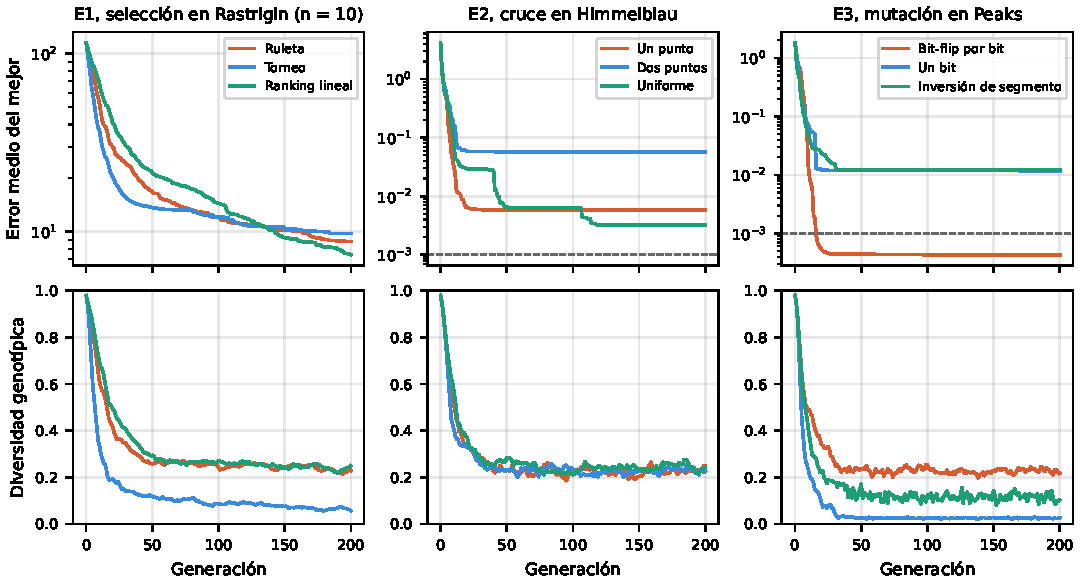
\includegraphics[width=\textwidth]{convergencia_experimentos.pdf}
\caption{Arriba, error del mejor individuo respecto al óptimo, promediado en las diez ejecuciones de cada variante, con la tolerancia de $10^{-3}$ punteada en E2 y E3. Abajo, diversidad genotípica media de la población. En E3 las curvas de error de un bit y de inversión de segmento casi se superponen.}
\label{fig:convergencia}
\end{figure*}

La Tabla~\ref{tab:metricas} reúne las métricas y la Fig.~\ref{fig:convergencia} las curvas promedio.

\textit{E1.} Ninguna variante alcanzó $10^{-3}$ en 200 generaciones. En la generación 25 el torneo llevaba el menor error (\EunoMejorTorneoGenVeinticinco{} frente a \EunoMejorRuletaGenVeinticinco{} de la ruleta y \EunoMejorRankingGenVeinticinco{} del ranking lineal, Kruskal-Wallis \EunoKruskalGenVeinticincoP) y ya había perdido diversidad (\EunoDivTorneoGenVeinticinco{} frente a \EunoDivRuletaGenVeinticinco{} y \EunoDivRankingGenVeinticinco). Desde la generación \EunoCruceRankingTorneo{} el ranking lineal tiene el menor error medio. El valor final no difiere entre métodos (\EunoKruskalP), y los tres seguían mejorando cerca de la generación 200. La diversidad final sí difiere, \EunoDivTorneoGenDoscientos{} en el torneo frente a \EunoDivRankingGenDoscientos{} en el ranking lineal (Mann-Whitney \EunoDivMannP).

\textit{E2.} El cruce de un punto alcanzó la tolerancia en 6 ejecuciones, el uniforme en 5 y el de dos puntos en 3. Sus medianas de generaciones fueron \EdosMedianaUnPunto, \EdosMedianaUniforme{} y \EdosMedianaDosPuntos, sin diferencia significativa (\EdosKruskalGenP). La diversidad final tampoco difiere (\EdosKruskalDivP). Las \EdosExitos{} ejecuciones con éxito terminaron en $(3, 2)$ o en $(3.58, -1.85)$, y las \EdosCercaDosTres{} que quedaron junto a los otros dos óptimos se detuvieron antes de la tolerancia. Ninguna de las \EdosSinExito{} ejecuciones sin éxito mejora cambiando un solo bit. Su cromosoma con éxito más cercano en el dominio está a una mediana de \EdosPasosMediana{} pasos de la rejilla, pero difiere en \EdosHammingCercanoMediana{} bits, cuando dos puntos al azar con el mismo desplazamiento difieren en \EdosHammingAzarMediana. El más cercano en bits está a \EdosHammingMin{} o más.

\textit{E3.} Bit-flip por bit alcanzó la tolerancia en las 10 ejecuciones, y un bit e inversión de segmento en 6 (Fisher \EtresFisherP). Su error medio fue $4.3\times10^{-4}$ frente a 0.0118 y 0.0120, y su diversidad final 0.22 frente a 0.03 y 0.10 (Mann-Whitney con un bit \EtresDivMannP). Ninguna ejecución de un bit sin éxito mejora cambiando un solo bit. El cromosoma con éxito más cercano en el dominio difiere en \EtresHammingCercanoMediana{} bits, frente a \EtresHammingAzarMediana{} al azar.

\section{Discusión}

E1 sigue a la presión selectiva. El torneo con $k=3$ reproduce casi solo a los mejores, explota antes la región hallada y pierde diversidad. El ranking lineal con $s=1.5$ da al mejor 1.5 veces la probabilidad media y explora más tiempo. La presión de la ruleta depende de la dispersión de la aptitud en cada generación, y queda en medio. Como las curvas seguían bajando, la convergencia prematura del torneo se ve en su diversidad y todavía no en su valor final.

En E2 el cruce de un punto conserva juntos los bits contiguos de cada variable, lo que es compatible con su menor mediana. El uniforme, el más disruptivo, no mostró más diversidad. Con diez ejecuciones estas diferencias no son significativas. Las ejecuciones sin éxito comparten un rasgo de la codificación. Quedan cerca del éxito en el dominio y lejos en bits, el patrón de los acantilados de Hamming \cite{caruana1988}. Con $P_m=1/32$, bit-flip por bit cambia un conjunto dado de 2 bits con probabilidad $\ProbConcretosDos$ por hijo, unas \EsperadoConcretosDos{} veces por ejecución como máximo, y uno de 5 bits con probabilidad $\ProbConcretosCinco$. Esas distancias quedan fuera de su alcance.

En E3 cuenta cuántos bits cambia cada mutación. Bit-flip por bit cambia en promedio uno por hijo, y dos o más con probabilidad \ProbDosBits, y mantiene la exploración. La de un bit nunca cambia más de uno y actúa solo en el 20~\% de los hijos, así que, una vez estancada, la búsqueda queda en explotación. La inversión de segmento da saltos mayores, pero conserva la cantidad de unos del cromosoma. Con los valores por defecto de la guía, la comparación mezcla la forma de cada mutación con su intensidad.

\section{Conclusiones}

La aplicación separa el motor de la interfaz, permite elegir desde la ventana los nueve operadores y todos los parámetros, y reproduce cada resultado con su semilla. En Rastrigin el torneo acelera el inicio a costa de la diversidad, sin cambiar el valor final a las 200 generaciones. En Himmelblau ningún cruce se distingue con diez ejecuciones, y ninguna ejecución alcanzó la tolerancia junto a dos de los cuatro óptimos. En Peaks bit-flip por bit fue la única mutación con éxito en todas las ejecuciones, lo que es compatible con su capacidad de cambiar varios bits a la vez.

\section*{Declaración de uso de inteligencia artificial}

Se usó Claude como apoyo en la redacción, la revisión de consistencia entre conceptos y la preparación de tablas y gráficas. Los procedimientos, el código fuente y la estructura del documento son del autor, quien verificó cada cifra con las salidas de los guiones de experimentos.

\begin{thebibliography}{99}
\bibitem{holland1975} J. H. Holland, \emph{Adaptation in Natural and Artificial Systems}. Ann Arbor, MI: University of Michigan Press, 1975.
\bibitem{goldberg1989} D. E. Goldberg, \emph{Genetic Algorithms in Search, Optimization, and Machine Learning}. Reading, MA: Addison-Wesley, 1989.
\bibitem{eiben2015} A. E. Eiben y J. E. Smith, \emph{Introduction to Evolutionary Computing}, 2.ª ed. Berlín: Springer, 2015, doi: \url{10.1007/978-3-662-44874-8}.
\bibitem{guia2026} Inteligencia Computacional Aplicada, ``Guía del proyecto, interfaz parametrizable para algoritmos genéticos,'' Universidad Distrital Francisco José de Caldas, 2026.
\bibitem{michalewicz1996} Z. Michalewicz, \emph{Genetic Algorithms + Data Structures = Evolution Programs}, 3.ª ed. Berlín: Springer, 1996, doi: \url{10.1007/978-3-662-03315-9}.
\bibitem{surjanovic} S. Surjanovic y D. Bingham, ``Virtual library of simulation experiments, test functions and datasets,'' Simon Fraser University. [En línea]. Disponible: \url{https://www.sfu.ca/~ssurjano/optimization.html}. Consultado: 19 nov. 2026.
\bibitem{peaks} MathWorks, ``peaks, Peaks function,'' documentación de MATLAB. [En línea]. Disponible: \url{https://www.mathworks.com/help/matlab/ref/peaks.html}. Consultado: 19 nov. 2026.
\bibitem{syswerda1989} G. Syswerda, ``Uniform crossover in genetic algorithms,'' en \emph{Proc. 3rd Int. Conf. Genetic Algorithms}, J. D. Schaffer, Ed. San Mateo, CA: Morgan Kaufmann, 1989, pp. 2--9.
\bibitem{harris2020} C. R. Harris \emph{et al.}, ``Array programming with NumPy,'' \emph{Nature}, vol. 585, pp. 357--362, 2020, doi: \url{10.1038/s41586-020-2649-2}.
\bibitem{pyside6} The Qt Company, ``Qt for Python (PySide6),'' licencia LGPL v3. [En línea]. Disponible: \url{https://doc.qt.io/qtforpython-6/}. Consultado: 22 nov. 2026.
\bibitem{hunter2007} J. D. Hunter, ``Matplotlib: A 2D graphics environment,'' \emph{Comput. Sci. Eng.}, vol. 9, n.º 3, pp. 90--95, 2007, doi: \url{10.1109/MCSE.2007.55}.
\bibitem{geatbx} H. Pohlheim, ``GEATbx examples, examples of objective functions,'' versión 3.8, 2006. [En línea]. Disponible: \url{http://www.geatbx.com}
\bibitem{pyinstaller} PyInstaller Development Team, ``PyInstaller,'' licencia GPL 2.0 con excepción de distribución. [En línea]. Disponible: \url{https://pyinstaller.org}. Consultado: 22 nov. 2026.
\bibitem{caruana1988} R. A. Caruana y J. D. Schaffer, ``Representation and hidden bias: Gray vs. binary coding for genetic algorithms,'' en \emph{Machine Learning Proceedings 1988}. San Mateo, CA: Morgan Kaufmann, 1988, pp. 153--161, doi: \url{10.1016/B978-0-934613-64-4.50021-9}.
\end{thebibliography}

\end{document}
